\section{Theorie}
\label{sec:Theorie}

\subsection{Aufbau einer Kathodenstrahlröhre}
Für den in den Versuchen benötigten Elektronenstrahl wird eine Kathodenstrahlröhre verwendet, welche aus drei Baugruppen zusammengesetzt ist.

\begin{figure}[h!]
	\centering
	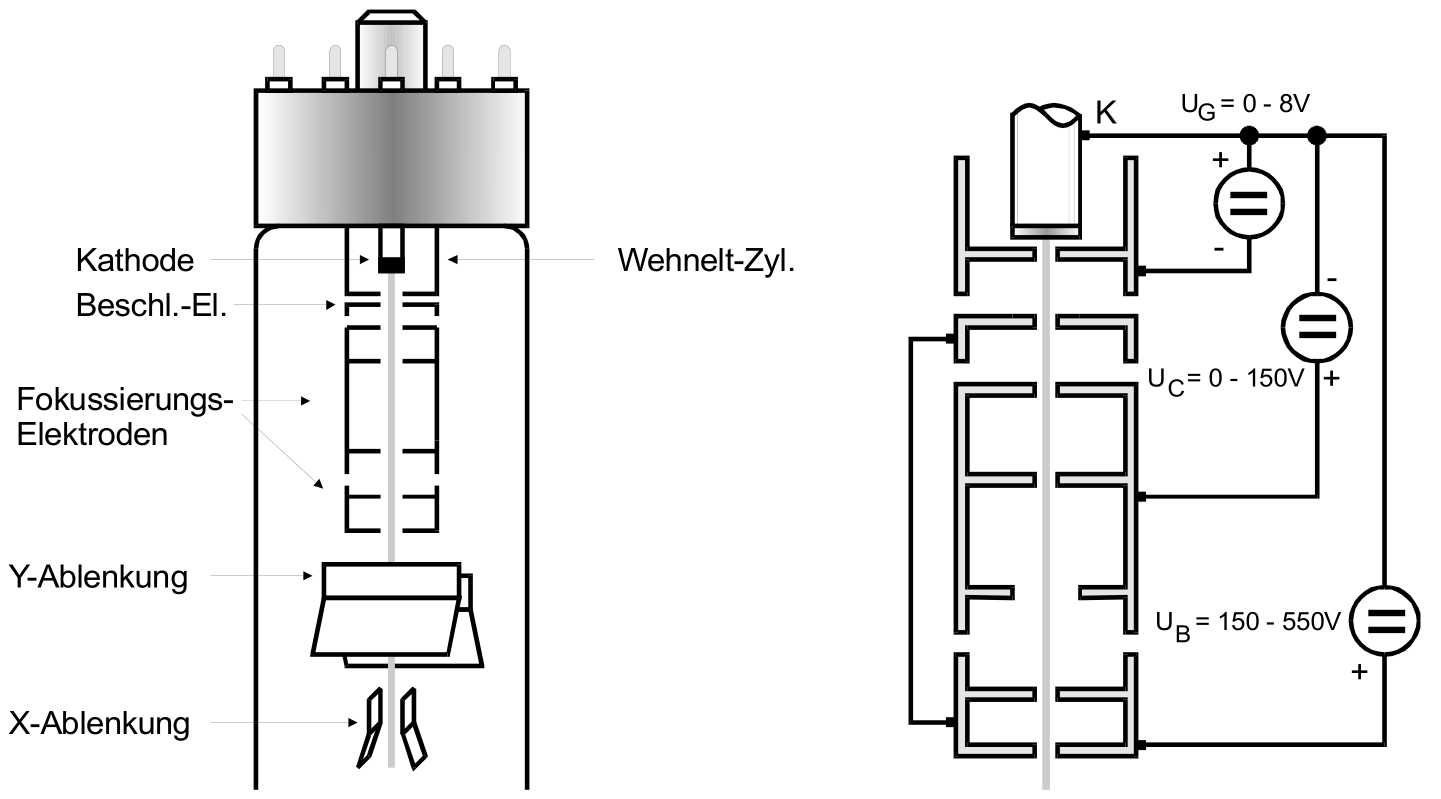
\includegraphics[width=0.9\linewidth]{../../kathodeaufbau}
	\caption{Aufbau der Kathodenstrahlröhre und Verschaltung der Elektronenkanone, \cite[2]{anleitung501}.}
	\label{fig:kathodeaufbau}
\end{figure}


Zunächst ist eine sogenannte Elektronenkanone zu finden. Diese besteht aus einer Glühkathode, die durch einen erhitzten isolierten Draht geheizt wird und Elektronen emittiert. Ein Wehnelt-Zylinder mit negativem
Potential umschließt die Kathode und sorgt dafür, dass die Intensität des austretenden Elektronenstrahls regelbar ist. Neben der umschlossenen Glühkathode ist eine Elektrode
angebracht, die mit ihrem starken positiven Potential $U_{\text{B}}$ die Elektronen auf eine Geschwindigkeit $v_{\text{z}}$ beschleunigt. Die Berechnung erfolgt mit dem Energiesatz:

\begin{equation}
\frac{m_0 v_{\text{z}}^2}{2} = e_0 U_{\text{B}}.
\label{eqn:energiesatz}
\end{equation}

Zur Bündelung des Strahls werden weitere Elektroden als eine Art Linse eingesetzt. Inhomogene Felder zwischen den Elektroden fokussieren den Strahl, mithilfe der angelegten Spannung $U_{\text{c}}$
kann die Brechkraft eingestellt werden. 

\begin{figure}[h!]
	\centering
	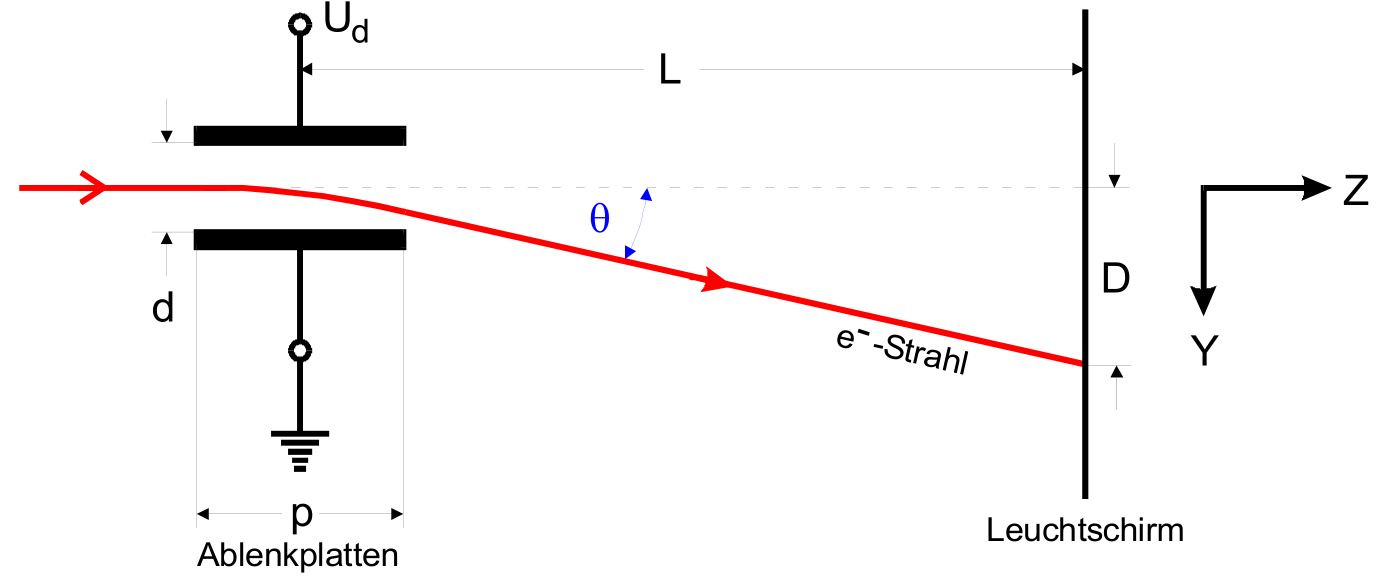
\includegraphics[width=0.9\linewidth]{../../AblenkungEFeld}
	\caption{Ablenkung des Elektronenstrahls im elektrischen Feld, \cite[3]{anleitung501}.}
	\label{fig:ablenkungefeld}
\end{figure}

Den zweiten Teil der Kathodenstrahlröhre stellt das Ablenksystem dar, das aus zwei Plattenpaaren zusammengesetzt ist. Eine angelegte Spannung $U_{\text{d}}$ erzeugt ein elektrisches Feld zwischen den 
Platten, das eine Kraft auf die hindurchtretenden Elektronen ausübt. Auf diese Weise kann der Elektronenstrahl je nach Spannung $U_{\text{d}}$ abgelenkt werden.

Der letzte Teil der Röhre ist der Leuchtschirm. Dieser weist die Auftreffstelle des Elektronenstrahls als leuchtenden Fleck nach.

\subsection{Berechnung der Ablenkung des Elektronenstrahls im elektrischen Feld}
Durch die an die Platten angelegte Spannung $U_{\text{d}}$ wird bei einem kleinen Plattenabstand $d$ bei großer Plattenlänge $p$  (Vgl. Abbildung \ref{fig:ablenkungefeld})
ein annähernd homogenes elektrisches Feld erzeugt. In diesem Feld wirkt auf das eintreffende Elektron eine Kraft, das abhängig von der Stärke des Feldes ist. Also gilt:

\begin{equation}
E = \frac{U_{\text{d}}}{d}
\end{equation}
und
\begin{equation}
|{F}| = |{e_0 \vec{E}}| = e_0 \frac{U_{\text{d}}}{d}.
\end{equation}
Die Kraft führt zu einer gleichmäßigen Beschleunigung in Y-Richtung. Die Geschwindigkeit lässt sich mithilfe der Kraft und des E-Feldes berechnen:

\begin{equation}
v_{\text{y}} = a_{\text{y}} \symup{\Delta{t}} = \frac{F}{m_0} \symup{\Delta{t}} = \frac{e_0}{m_0} \frac{U_{\text{d}}}{d} \symup{\Delta{t}}.
\label{eqn:vy}
\end{equation}
Weiterhin hat das Elektron eine Geschwindigkeitskomponente $v_{\text{z}}$ in Z-Richtung. Damit gilt für die Zeit $\symup{\Delta{t}}$, für die sich das Elektron im Feld befindet:

\begin{equation}
\symup{\Delta{t}} = \frac{p}{v_{\text{z}}}.
\end{equation}
Durch Einsetzen in Gleichung \ref{eqn:vy} ergibt sich dann für die Geschwindigkeit in Y-Richtung:

\begin{equation}
v_{\text{y}} = \frac{e_0}{m_0} \frac{U_{\text{d}}}{d} \frac{p}{v_{\text{z}}}.
\end{equation}

Die Verschiebung des Leuchtflecks auf dem Schirm lässt sich ermitteln über den Abstand der Platten zum Schirm und dem Winkel $\theta$, um den der Strahl abgelenkt wird.
Der Winkel lässt sich mithilfe der beiden Geschwindigkeitskomponenten berechnen:

\begin{equation}
\begin{aligned}
\theta &\cong \frac{v_{\text{y}}}{v_{\text{z}}}
\implies \theta = \frac{e_0}{m_0} \frac{U_{\text{d}}}{d} \frac{p}{v_{\text{z}}^2}.
\end{aligned}
\end{equation}
Damit ist die Verschiebung $D$:

\begin{equation}
D = L \cdot \theta = L \cdot \frac{e_0}{m_0} \frac{U_{\text{d}}}{d} \frac{p}{v_{\text{z}}^2}.
\label{eqn:verschiebung}
\end{equation}

Wird die Energiesatzgleichung \ref{eqn:energiesatz} nach $v_{\text{z}}^2$ umgestellt und in Gleichung \ref{eqn:verschiebung} eingesetzt, so lässt sich die Veschiebung $D$ auf dem Schirm auch mit:

\begin{equation}
D = L \cdot \frac{p}{2d} \frac{U_{\text{d}}}{U_{\text{B}}}
\end{equation}
berrechnen. Neben der Abhängigkeit von der Beschleunigungsspannung $U_{\text{B}}$ und den Maßen des Kondensator ist auch ein Proportionalitätfaktor zwischen $D$ und der Ablenkspannung $U_{\text{d}}$ zu erkennen, welcher auch als Empfindlichkeit bezeichnet wird. Dabei ist es wichtig zu nennen, dass je kleiner die Ablenkspannung, desto größer wird die Beschleunigungsspannung.
Für eine hohe Empfindlichkeit müssen einige Bedingungen gelten und zwar eine großen Strahlweg L, eine kleine Beschleunigungsspannung und einen langen Ablenkkondensator p.

\subsection{Prinzip des Kathodenstrahl-Oszillographen}
Bei einem Kathodenstrahl-Oszillographen wird eine Kathodenstrahlröhre eingesetzt und wird für die zeitliche Darstellung von Wechselspannungen verwendet. Hierzu wird an das in X-Richtung ablenkende Plattenpaar 
eine Sägezahnspannung angelegt und an das in Y-Richtung ablenkende eine Spannung, die untersucht werden soll. Aus diesen Spannungen lassen sich auf dem Leuchtschirm stehende Wellen erzeugen, die bei bestimmten Frequenzen entstehen, sofern für die 
Frequenzen die Synchronisationsbedingung:

\begin{equation}
n\cdot \nu_{\text{Sä}} = m \cdot \nu_{\text{We}}
\end{equation}
gilt, mit $n = 1,2,3,...$ und $m = 1,2,3,...$


Für die Erzeugung stehender Wellen gilt als Voraussetzung, dass sie bei gleicher Frequenz und gleicher Amplitude aus einer hin- und rücklaufende Welle entstehen. Zum anderen besitzen stehende Wellen Schwingungsknoten. Dort bleiben sie in Ruhe und findet keine Auslenkung statt. Eine maximale Auslenkung wird durch den Schwingungsbauch erzeugt, wenn sie sich in der Mitte treffen. 